\documentclass[11pt,a4paper]{report}
\usepackage[textwidth=37em,vmargin=30mm]{geometry}
\usepackage{calc,xunicode,amsmath,amssymb,paralist,enumitem,tabu,booktabs,datetime2,xeCJK,xeCJKfntef,listings}
\usepackage{tocloft,fancyhdr,tcolorbox,xcolor,graphicx,eso-pic,xltxtra,xelatexemoji}

\newcommand{\envyear}[0]{2025}
\newcommand{\envdatestr}[0]{2025-09-15}
\newcommand{\envfinaldir}[0]{webdb/2025/20250915/final}

\usepackage[hidelinks]{hyperref}
\hypersetup{
    colorlinks=false,
    pdfpagemode=FullScreen,
    pdftitle={Web Digest - \envdatestr}
}

\setlength{\cftbeforechapskip}{10pt}
\renewcommand{\cftchapfont}{\rmfamily\bfseries\large\raggedright}
\setlength{\cftbeforesecskip}{2pt}
\renewcommand{\cftsecfont}{\sffamily\small\raggedright}

\setdefaultleftmargin{2em}{2em}{1em}{1em}{1em}{1em}

\usepackage{xeCJK,xeCJKfntef}
\xeCJKsetup{PunctStyle=plain,RubberPunctSkip=false,CJKglue=\strut\hskip 0pt plus 0.1em minus 0.05em,CJKecglue=\strut\hskip 0.22em plus 0.2em}
\XeTeXlinebreaklocale "zh"
\XeTeXlinebreakskip = 0pt


\setmainfont{Brygada 1918}
\setromanfont{Brygada 1918}
\setsansfont{IBM Plex Sans}
\setmonofont{JetBrains Mono NL}
\setCJKmainfont{Noto Serif CJK SC}
\setCJKromanfont{Noto Serif CJK SC}
\setCJKsansfont{Noto Sans CJK SC}
\setCJKmonofont{Noto Sans CJK SC}

\setlength{\parindent}{0pt}
\setlength{\parskip}{8pt}
\linespread{1.15}

\lstset{
	basicstyle=\ttfamily\footnotesize,
	numbersep=5pt,
	backgroundcolor=\color{black!5},
	showspaces=false,
	showstringspaces=false,
	showtabs=false,
	tabsize=2,
	captionpos=b,
	breaklines=true,
	breakatwhitespace=true,
	breakautoindent=true,
	linewidth=\textwidth
}






\newcommand{\coverpic}[2]{
    % argv: itemurl, authorname
    Cover photo by #2~~(\href{#1}{#1})
}
\newcommand{\makeheader}[0]{
    \begin{titlepage}
        % \newgeometry{hmargin=15mm,tmargin=21mm,bmargin=12mm}
        \begin{center}
            
            \rmfamily\scshape
            \fontspec{BaskervilleF}
            \fontspec{Old Standard}
            \fontsize{59pt}{70pt}\selectfont
            WEB\hfill DIGEST
            
            \vfill
            % \vskip 30pt
            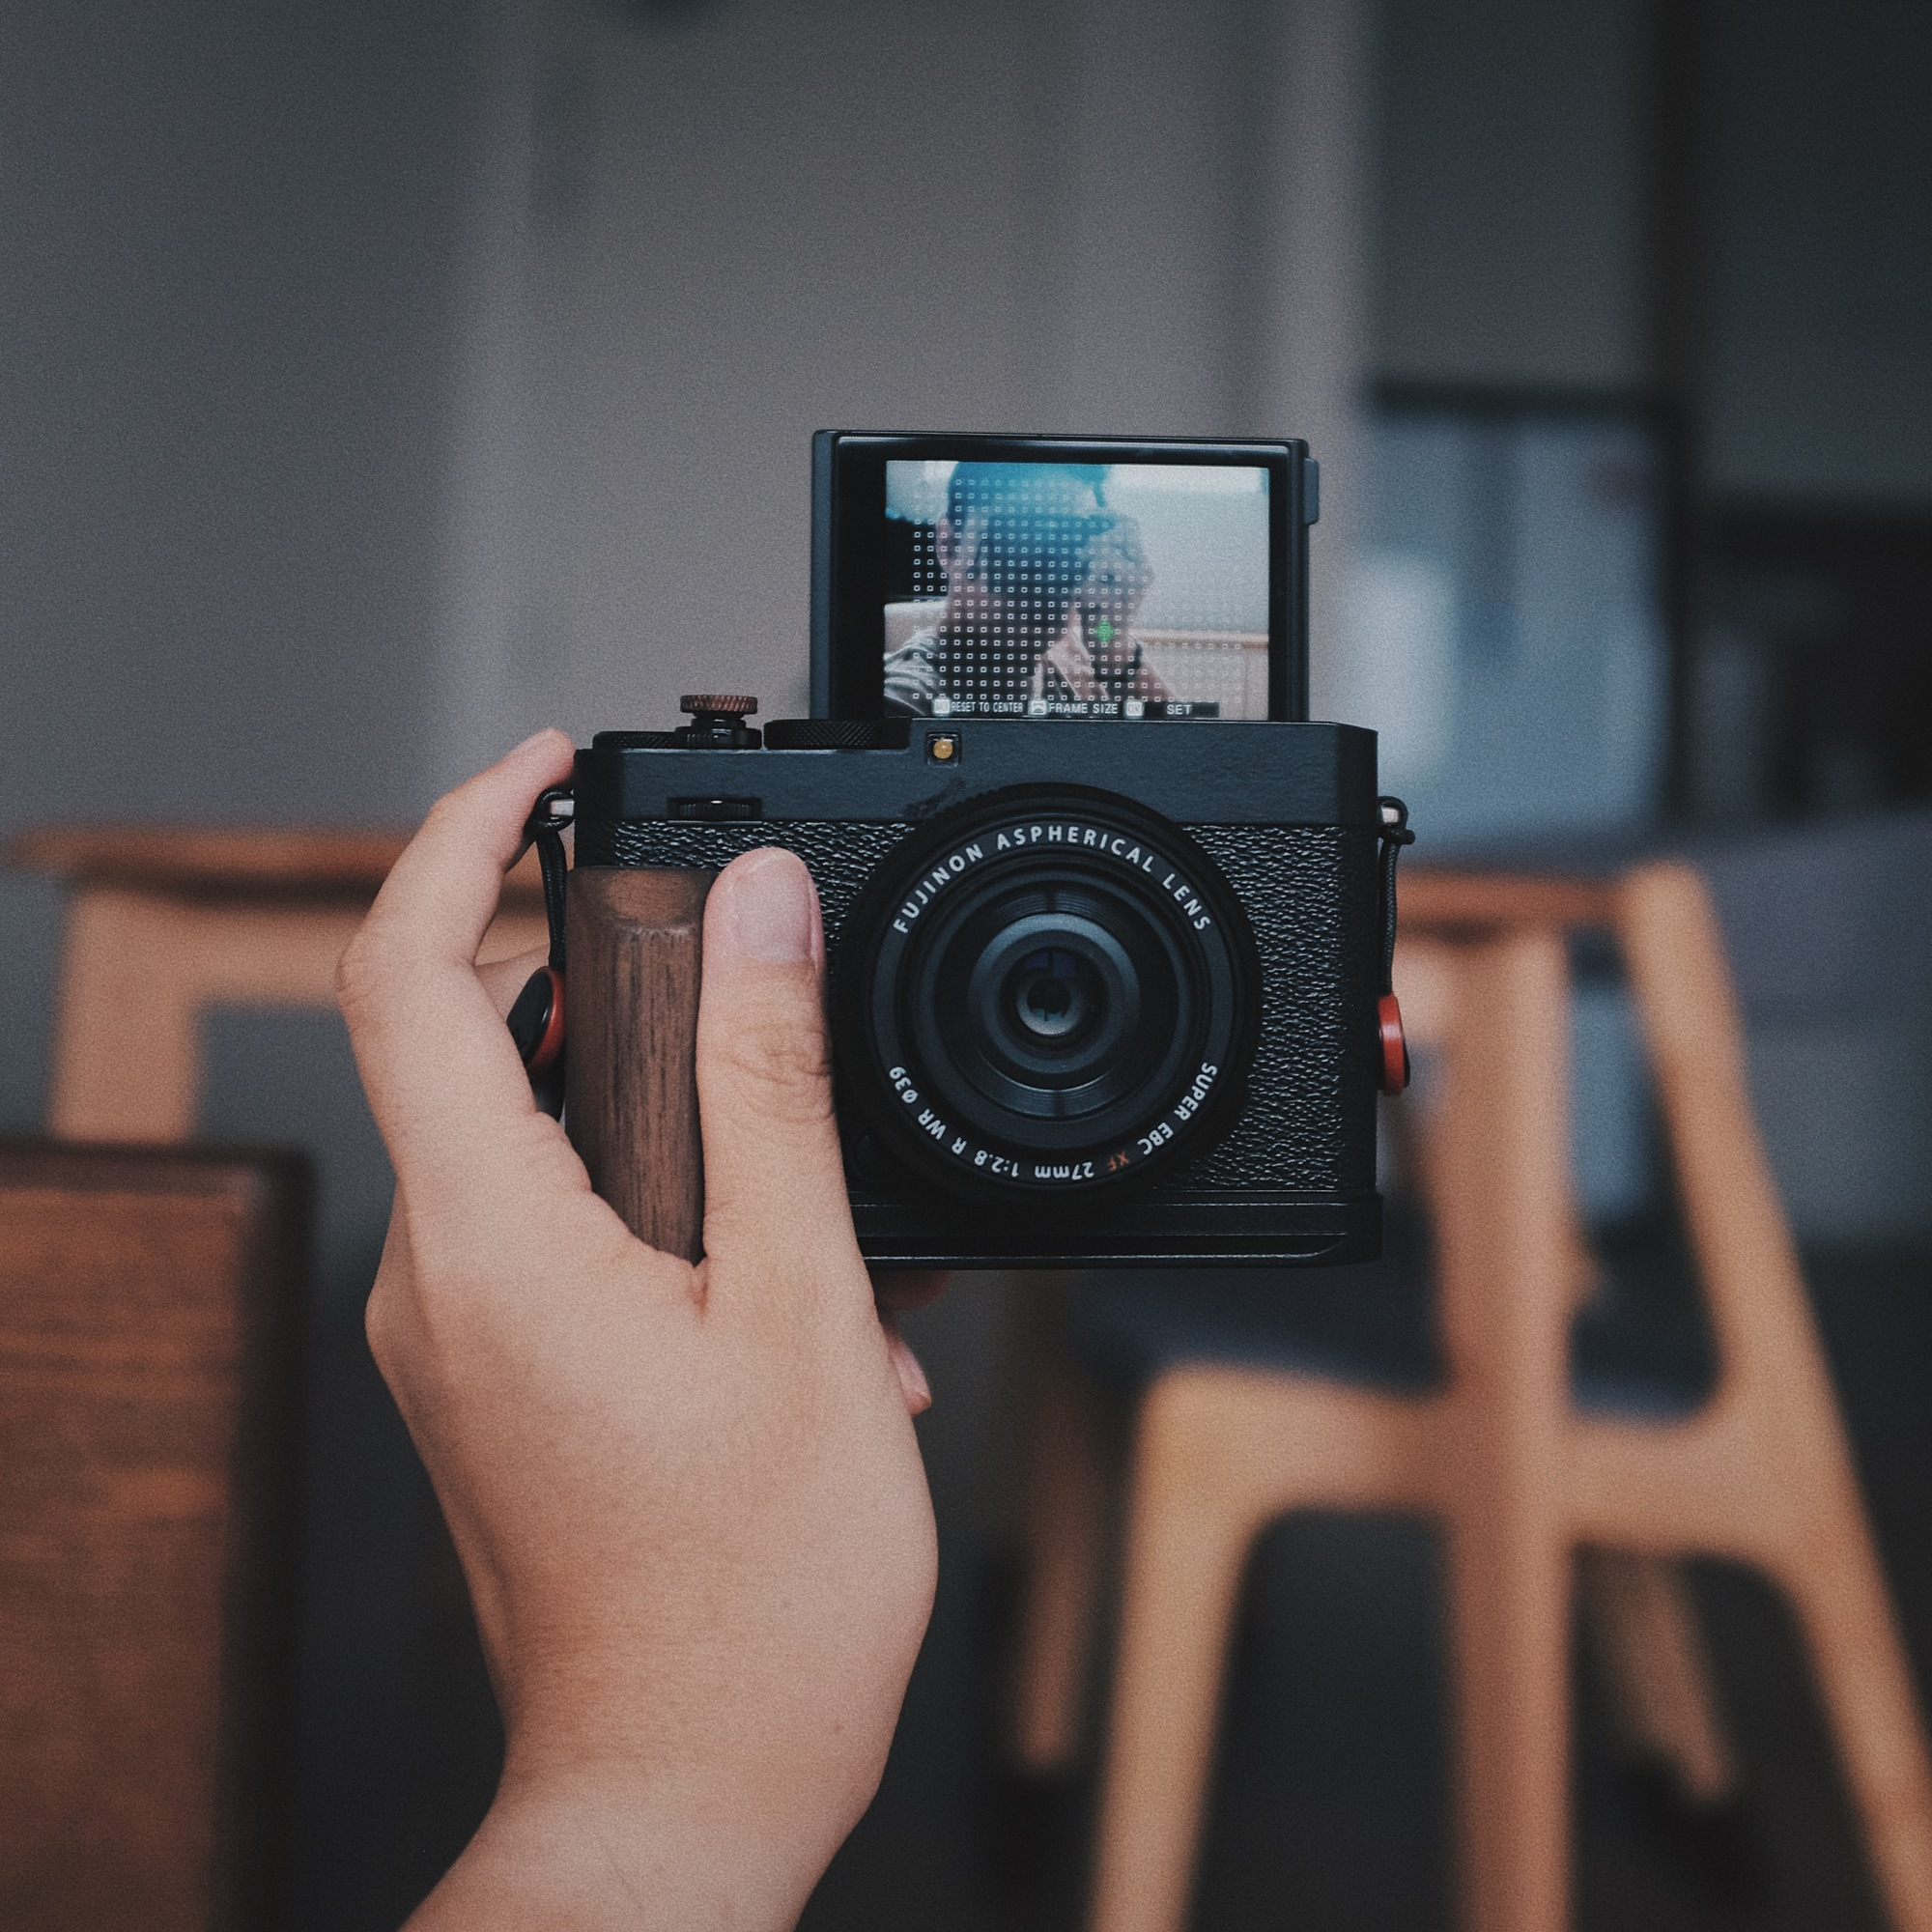
\includegraphics[width=\linewidth]{\envfinaldir/coverpic-prod.jpg}\par
            % \vskip 30pt
            \vfill

            \normalsize\rmfamily\scshape
            \copyright{} The Web Digest Project \hfill\large \envdatestr
        \end{center}
    \end{titlepage}
    % \restoregeometry
}
\newcommand{\simplehref}[1]{%
    \textcolor{blue!80!green}{\href{#1}{#1}}%
}
\renewcommand{\contentsname}{\center\Huge\sffamily\bfseries Contents\par\vskip 20pt}
\newcounter{ipartcounter}
\setcounter{ipartcounter}{0}
\newcommand{\ipart}[1]{
    % \vskip 20pt
    \clearpage
    \stepcounter{ipartcounter}
    \phantomsection
    \addcontentsline{toc}{chapter}{#1}
    % \begin{center}
    %     \Huge
    %     \sffamily\bfseries
    %     #1
    % \end{center}
    % \vskip 20pt plus 7pt
}
\newcounter{ichaptercounter}
\setcounter{ichaptercounter}{0}
\newcommand{\ichapter}[1]{
    % \vskip 20pt
    \clearpage
    \stepcounter{ichaptercounter}
    \phantomsection
    \addcontentsline{toc}{section}{\numberline{\arabic{ichaptercounter}}#1}
    \begin{center}
        \Huge
        \sffamily\bfseries
        #1
    \end{center}
    \vskip 20pt plus 7pt
}
\newcommand{\entrytitlefont}[1]{\subsection*{\raggedright\Large\sffamily\bfseries#1}}
\newcommand{\entryitemGeneric}[2]{
    % argv: title, url
    \parbox{\linewidth}{
        \entrytitlefont{#1}\par\vskip 5pt
        \footnotesize\ttfamily\mdseries
        \simplehref{#2}
    }\vskip 11pt plus 11pt minus 1pt
}
\newcommand{\entryitemGithub}[3]{
    % argv: title, url, desc
    \parbox{\linewidth}{
        \entrytitlefont{#1}\par\vskip 5pt
        \footnotesize\ttfamily\mdseries
        \simplehref{#2}\par\vskip 5pt
        \small\rmfamily\mdseries#3
    }\vskip 11pt plus 11pt minus 1pt
}
\newcommand{\entryitemAp}[3]{
    % argv: title, url, desc
    \parbox{\linewidth}{
        \entrytitlefont{#1}\par\vskip 5pt
        \footnotesize\ttfamily\mdseries
        \simplehref{#2}\par\vskip 5pt
        \small\rmfamily\mdseries#3
    }\vskip 11pt plus 11pt minus 1pt
}
\newcommand{\entryitemHackernews}[3]{
    % argv: title, hnurl, rawurl
    % \parbox{\linewidth}{
    %     \entrytitlefont{#1}\par\vskip 5pt
    %     \footnotesize\ttfamily\mdseries
    %     \simplehref{#3}\par
    %     \textcolor{black!50}{\href{#2}{#2}}
    % }\vskip 11pt plus 11pt minus 1pt
    \begin{minipage}{\linewidth}
            \entrytitlefont{#1}\par\vskip 5pt
            \footnotesize\ttfamily\mdseries
            \simplehref{#3}\par
            \textcolor{black!50}{\href{#2}{#2}}
    \end{minipage}\par\vskip 11pt plus 11pt minus 1pt
}







\begin{document}

\makeheader

\tableofcontents\clearpage




\ipart{Developers}
\ichapter{Hacker News}
\entryitemTwoLinks{ChatControl update: blocking minority held but Denmark is moving forward anyway}{https://news.ycombinator.com/item?id=45242458}{https://disobey.net/@yawnbox/115203365485529363}

\entryitemTwoLinks{Writing an operating system kernel from scratch}{https://news.ycombinator.com/item?id=45240682}{https://popovicu.com/posts/writing-an-operating-system-kernel-from-scratch/}

\entryitemTwoLinks{Nicu's test website made with SVG (2007)}{https://news.ycombinator.com/item?id=45240391}{https://svg.nicubunu.ro/}

\entryitemTwoLinks{Bank of Thailand freezes 3M accounts, sets daily transfer limits to curb fraud}{https://news.ycombinator.com/item?id=45240304}{https://www.thaienquirer.com/57752/bot-freezes-3-million-accounts-sets-daily-transfer-limits-of-50000-200000-baht-to-curb-6-billion-baht-scam-losses/}

\entryitemTwoLinks{Why We Spiral}{https://news.ycombinator.com/item?id=45240146}{https://behavioralscientist.org/why-we-spiral/}

\entryitemTwoLinks{EPA Seeks to Eliminate Critical PFAS Drinking Water Protections}{https://news.ycombinator.com/item?id=45239803}{https://earthjustice.org/press/2025/epa-seeks-to-roll-back-pfas-drinking-water-rules-keeping-millions-exposed-to-toxic-forever-chemicals-in-tap-water}

\entryitemTwoLinks{Read to forget}{https://news.ycombinator.com/item?id=45239601}{https://mo42.bearblog.dev/read-to-forget/}

\entryitemTwoLinks{Repetitive negative thinking associated with cognitive decline in older adults}{https://news.ycombinator.com/item?id=45239085}{https://bmcpsychiatry.biomedcentral.com/articles/10.1186/s12888-025-06815-2}

\entryitemTwoLinks{macOS Tahoe is certified Unix 03 [pdf]}{https://news.ycombinator.com/item?id=45238930}{https://www.opengroup.org/openbrand/certificates/1223p.pdf}

\entryitemTwoLinks{Fukushima insects tested for cognition}{https://news.ycombinator.com/item?id=45238836}{https://news.cnrs.fr/articles/fukushima-insects-tested-for-cognition}

\entryitemTwoLinks{Models of European metro stations}{https://news.ycombinator.com/item?id=45238055}{http://stations.albertguillaumes.cat/}

\entryitemTwoLinks{Cat Aquariums}{https://news.ycombinator.com/item?id=45237970}{https://cataquariums.com/}

\entryitemTwoLinks{SpikingBrain 7B – More efficient than classic LLMs}{https://news.ycombinator.com/item?id=45237754}{https://github.com/BICLab/SpikingBrain-7B}

\entryitemTwoLinks{Refurb Weekend: Silicon Graphics Indigo² Impact 10000}{https://news.ycombinator.com/item?id=45237717}{http://oldvcr.blogspot.com/2025/09/refurb-weekend-silicon-graphics-indigo.html}

\entryitemTwoLinks{A single, 'naked' black hole confounds theories of the young cosmos}{https://news.ycombinator.com/item?id=45237442}{https://www.quantamagazine.org/a-single-naked-black-hole-rewrites-the-history-of-the-universe-20250912/}

\entryitemTwoLinks{How the restoration of ancient Babylon is drawing tourists back to Iraq}{https://news.ycombinator.com/item?id=45236473}{https://www.theartnewspaper.com/2025/09/12/how-the-restoration-of-ancient-babylon-is-helping-to-draw-tourists-back-to-iraq}

\entryitemTwoLinks{If my kids excel, will they move away?}{https://news.ycombinator.com/item?id=45236411}{https://jeffreybigham.com/blog/2025/where-will-my-kids-go.html}

\entryitemTwoLinks{EFF to court: The Supreme Court must rein in secondary copyright liability}{https://news.ycombinator.com/item?id=45236314}{https://www.eff.org/deeplinks/2025/09/eff-court-supreme-court-must-rein-expansive-secondary-copyright-liability}

\entryitemTwoLinks{Two Slice, a font that's only 2px tall}{https://news.ycombinator.com/item?id=45236263}{https://joefatula.com/twoslice.html}

\entryitemTwoLinks{Pass: Unix Password Manager}{https://news.ycombinator.com/item?id=45236079}{https://www.passwordstore.org/}\ichapter{Phoronix}
\entryitemGeneric{\hskip 0pt{}Linux 6.17-rc6 Released With VMSCAPE Mitigation, FLYDIGI APEX 5 Support \& Fixes}{https://www.phoronix.com/news/Linux-6.17-rc6-Released}

\entryitemGeneric{\hskip 0pt{}Intel Loses One Of Its USB4 / Thunderbolt Linux Driver Maintainers}{https://www.phoronix.com/news/USB4-Thunderbolt-Maintainer}

\entryitemGeneric{\hskip 0pt{}FLYDIGI APEX 5 Controller Support Landing In Linux 6.17}{https://www.phoronix.com/news/FLYDIGI-APEX-5-Linux-6.17}

\entryitemGeneric{\hskip 0pt{}Select Qualcomm X Elite Laptops Seeing IRIS Video Acceleration On Linux}{https://www.phoronix.com/news/Qualcomm-X-Elite-IRIS-Video}

\entryitemGeneric{\hskip 0pt{}Samsung Exynos 7870 Seeing New Open-Source Driver Activity For Linux 6.18}{https://www.phoronix.com/news/Samsung-Exynos-7870-Linux-6.18}

\entryitemGeneric{\hskip 0pt{}Redox OS To Focus More On Wayland, "Redox Server" \& Performance Over The Next Year}{https://www.phoronix.com/news/Redox-OS-2026-Plans}

\entryitemGeneric{\hskip 0pt{}Linux's New "Sheaves" Per-CPU Caching Layer Showing Massive Wins For AMD Performance}{https://www.phoronix.com/news/Linux-Sheaves-AMD-Performance}

\entryitemGeneric{\hskip 0pt{}Cloud Hypervisor Will Block AI Generated Code, Raises x86\_64 VM Limit To 8,192 vCPUs}{https://www.phoronix.com/news/Cloud-Hypervisor-48}

\entryitemGeneric{\hskip 0pt{}62 Patches Posted For Stripping Classic Initrd Support From The Linux Kernel}{https://www.phoronix.com/news/Patches-Remove-Classic-Initrd}


\ipart{Developers~~~~(zh-Hans)}
\ichapter{Solidot}
\entryitemGeneric{\hskip 0pt{}社交媒体的末日}{https://www.solidot.org/story?sid=82304}

\entryitemGeneric{\hskip 0pt{}互联网档案馆保存的网页数即将突破 1 万亿}{https://www.solidot.org/story?sid=82303}

\entryitemGeneric{\hskip 0pt{}尼泊尔 Z 世代抗议中的技术力量}{https://www.solidot.org/story?sid=82302}

\entryitemGeneric{\hskip 0pt{}Proton Mail 应网络安全机构要求关闭了记者账户}{https://www.solidot.org/story?sid=82301}

\entryitemGeneric{\hskip 0pt{}中国电动汽车技术如何重塑全球汽车设计}{https://www.solidot.org/story?sid=82300}

\entryitemGeneric{\hskip 0pt{}Apache 软件基金会使用新 Logo 和名字 ASF}{https://www.solidot.org/story?sid=82299}

\entryitemGeneric{\hskip 0pt{}大英百科和韦氏词典指控 Perplexity 侵犯版权和商标权}{https://www.solidot.org/story?sid=82298}

\entryitemGeneric{\hskip 0pt{}世嘉不小心卖掉了任天堂开发套件,恐惧下报警突击搜查买家}{https://www.solidot.org/story?sid=82297}

\entryitemGeneric{\hskip 0pt{}为打击腐败阿尔巴尼亚任命了一名 AI 部长}{https://www.solidot.org/story?sid=82296}

\entryitemGeneric{\hskip 0pt{}AirPods 实时翻译功能暂不向欧洲和中国大陆提供}{https://www.solidot.org/story?sid=82295}

\entryitemGeneric{\hskip 0pt{}全球消费的鳗鱼 99\% 属于濒危物种}{https://www.solidot.org/story?sid=82294}

\entryitemGeneric{\hskip 0pt{}矮行星鸟神星发现甲烷气体}{https://www.solidot.org/story?sid=82293}

\entryitemGeneric{\hskip 0pt{}章鱼有偏好使用的腕足}{https://www.solidot.org/story?sid=82292}

\entryitemGeneric{\hskip 0pt{}Windows 开发者可免费在 Microsoft Store 发布应用}{https://www.solidot.org/story?sid=82291}

\entryitemGeneric{\hskip 0pt{}Vimeo 以 13.8 亿美元出售给 Bending Spoons}{https://www.solidot.org/story?sid=82290}

\entryitemGeneric{\hskip 0pt{}Firefox 支持播放 MKV 内容}{https://www.solidot.org/story?sid=82289}\ichapter{V2EX}
\entryitemGeneric{\hskip 0pt{}[问与答] 各位,访问 gpt5 是不是需要特别干净的网络环境啊,某口用不了是不?}{https://www.v2ex.com/t/1159171}

\entryitemGeneric{\hskip 0pt{}[生活] 沟通问题,请大家帮忙分析}{https://www.v2ex.com/t/1159170}

\entryitemGeneric{\hskip 0pt{}[分享创造] Nano banana 图片编辑能力真是太强了}{https://www.v2ex.com/t/1159169}

\entryitemGeneric{\hskip 0pt{}[分享创造] 产品上线半月的故障、挑战与优化之路}{https://www.v2ex.com/t/1159168}

\entryitemGeneric{\hskip 0pt{}[iOS] 请问 Apple ID 港区是否用云上贵州,国内 app 广告肆无忌惮,想找个区下载国内 app 又无广告的}{https://www.v2ex.com/t/1159167}

\entryitemGeneric{\hskip 0pt{}[DotA] 赛点了家人们,紧张吗.....}{https://www.v2ex.com/t/1159164}

\entryitemGeneric{\hskip 0pt{}[问与答] 降息通道哪个赛道收益率会最高?}{https://www.v2ex.com/t/1159161}

\entryitemGeneric{\hskip 0pt{}[分享发现] 移动 无忧行 貌似上线了 eSIM}{https://www.v2ex.com/t/1159160}

\entryitemGeneric{\hskip 0pt{}[分享创造] 📢送兑换码换意见反馈了}{https://www.v2ex.com/t/1159159}

\entryitemGeneric{\hskip 0pt{}[Windows] win11 蓝屏, What failed: VMMRO.r0,大概率和 eNSP 使用有关}{https://www.v2ex.com/t/1159158}

\entryitemGeneric{\hskip 0pt{}[推广] 天翼云 45 折 腾讯云 阿里云 阿里云国际 AWS 大陆 3 折 需要的看过来~}{https://www.v2ex.com/t/1159157}

\entryitemGeneric{\hskip 0pt{}[分享发现] chrome 新版本的 split view 还是挺实用的}{https://www.v2ex.com/t/1159156}

\entryitemGeneric{\hskip 0pt{}[北京] [霍营] [西三旗] 房东自住房出租。小区最好的户型,精装修风水好。}{https://www.v2ex.com/t/1159154}

\entryitemGeneric{\hskip 0pt{}[投资] A 股超短,题材切换研究}{https://www.v2ex.com/t/1159153}

\entryitemGeneric{\hskip 0pt{}[问与答] 工行信用卡的境外无卡支付锁打开,会导致被盗刷吗?}{https://www.v2ex.com/t/1159152}

\entryitemGeneric{\hskip 0pt{}[问与答] 美区账号里有些购买的软件,能给家里人用吗}{https://www.v2ex.com/t/1159151}

\entryitemGeneric{\hskip 0pt{}[投资] 大 A 期货}{https://www.v2ex.com/t/1159150}

\entryitemGeneric{\hskip 0pt{}[分享创造] 正在制作一款 2D 像素版建岛游戏(仿动森)}{https://www.v2ex.com/t/1159149}

\entryitemGeneric{\hskip 0pt{}[iOS] iOS 端提示要求同意云上贵州协议,但是不影响继续使用,是什么情况?}{https://www.v2ex.com/t/1159148}

\entryitemGeneric{\hskip 0pt{}[创业组队] 🚀 寻找 AI 垂类赛道 技术合伙人}{https://www.v2ex.com/t/1159147}

\entryitemGeneric{\hskip 0pt{}[问与答] 关于孩子教育问题,商场遇到奇葩男孩有感}{https://www.v2ex.com/t/1159145}

\entryitemGeneric{\hskip 0pt{}[问与答] 有没有南方跟北方的来对下账,在东北教师节要给老师送礼,而南方不需要}{https://www.v2ex.com/t/1159143}

\entryitemGeneric{\hskip 0pt{}[Apple] 土区 iCloud 下个月涨价了,怎么迁移到国区来啊?}{https://www.v2ex.com/t/1159141}

\entryitemGeneric{\hskip 0pt{}[生活] 时间无法停,人生的路总是要抉择的。(记录不必回)}{https://www.v2ex.com/t/1159138}

\entryitemGeneric{\hskip 0pt{}[投资] 盈透是不是入金任何金额就算账户入金了?}{https://www.v2ex.com/t/1159136}

\entryitemGeneric{\hskip 0pt{}[问与答] mac 外接显示器疑问}{https://www.v2ex.com/t/1159135}

\entryitemGeneric{\hskip 0pt{}[问与答] giffgaff 收到 10085 和腾讯总部的电话?}{https://www.v2ex.com/t/1159134}

\entryitemGeneric{\hskip 0pt{}[Android] 分享安卓调节色彩饱和度的软件 sansgood/Sa2ration}{https://www.v2ex.com/t/1159133}

\entryitemGeneric{\hskip 0pt{}[问与答] 发现甲骨文云的流量消耗异常的大,各位遇到过吗,只是看看视频,一周就将近 150g}{https://www.v2ex.com/t/1159132}

\entryitemGeneric{\hskip 0pt{}[投资] 免五开户再不开就没了!需要万 0.7 免五的找我..}{https://www.v2ex.com/t/1159130}

\entryitemGeneric{\hskip 0pt{}[问与答] 今年的大闸蟹怎么还没来}{https://www.v2ex.com/t/1159129}

\entryitemGeneric{\hskip 0pt{}[Android] 202509 求推荐个安卓备用机}{https://www.v2ex.com/t/1159128}

\entryitemGeneric{\hskip 0pt{}[酷工作] 招聘: 法币出入金 产品经理 产品经理(交易平台) 产品经理(触达) RWA 产品经理 Golang 工程师(5-10 个 HC)}{https://www.v2ex.com/t/1159126}

\entryitemGeneric{\hskip 0pt{}[问与答] 提问有无好用的 ai 相册}{https://www.v2ex.com/t/1159125}

\entryitemGeneric{\hskip 0pt{}[问与答] 域名不备案的话会被干扰吗}{https://www.v2ex.com/t/1159123}

\entryitemGeneric{\hskip 0pt{}[分享创造] 写简历改到头秃?我做了个 AI 简历教练,让它手把手教你写出能打的简历}{https://www.v2ex.com/t/1159122}

\entryitemGeneric{\hskip 0pt{}[生活] 你们是什么时候第一次遇到过家人去世的,有什么反应}{https://www.v2ex.com/t/1159121}

\entryitemGeneric{\hskip 0pt{}[Apple] iPhone17 各国版本区别及购机讨论}{https://www.v2ex.com/t/1159120}

\entryitemGeneric{\hskip 0pt{}[小米] 如何说服小米售后回滚 MIUI?}{https://www.v2ex.com/t/1159119}

\entryitemGeneric{\hskip 0pt{}[问与答] 大家都是如何玩 ipv6 的}{https://www.v2ex.com/t/1159118}

\entryitemGeneric{\hskip 0pt{}[服务器] 服务器超融合及桌面云最终方案选择}{https://www.v2ex.com/t/1159117}

\entryitemGeneric{\hskip 0pt{}[Solana] 有没有买 PUMP 的?}{https://www.v2ex.com/t/1159116}

\entryitemGeneric{\hskip 0pt{}[投资] 合约跟单,兄弟们别嫌少,真的稳定}{https://www.v2ex.com/t/1159115}

\entryitemGeneric{\hskip 0pt{}[投资] 港股 8.19 日入金 10W 港 截至目前合计: 133548.63 港 我承认行情是主要的}{https://www.v2ex.com/t/1159114}

\entryitemGeneric{\hskip 0pt{}[macOS] 2020 款 M1 MacBook Pro 16GB,可上 macOS 26 吗?}{https://www.v2ex.com/t/1159113}

\entryitemGeneric{\hskip 0pt{}[魂系游戏] 丝之歌通关了}{https://www.v2ex.com/t/1159112}

\entryitemGeneric{\hskip 0pt{}[问与答] 千元内能拿下一个性能不错的 pixel 吗,或者是三星}{https://www.v2ex.com/t/1159111}

\entryitemGeneric{\hskip 0pt{}[分享创造] 我做了一个浏览器插件: CRT 扫描线特效模拟}{https://www.v2ex.com/t/1159110}

\entryitemGeneric{\hskip 0pt{}[iOS] iPadOS 26 游戏性能相比 iPadOS17 有下降吗?}{https://www.v2ex.com/t/1159109}

\entryitemGeneric{\hskip 0pt{}[Apple] 可能今年 iPhone17 基础款唯一的``缺点''就是高通基带了}{https://www.v2ex.com/t/1159108}


\ipart{Generic News}







\clearpage
\leavevmode\vfill
\footnotesize

Copyright \copyright{} 2023-2025 Neruthes and other contributors.

This document is published with CC BY-NC-ND 4.0 license.

The entries listed in this newsletter may be copyrighted by their respective creators.

This newsletter is generated by the Web Digest project.

The newsletters are also delivered via Telegram channel \CJKunderline{\href{https://t.me/webdigestchannel}{https://t.me/webdigestchannel}}.\\
RSS feed is available at \CJKunderline{\href{https://webdigest.pages.dev/rss.xml}{https://webdigest.pages.dev/rss.xml}}.

This newsletter is available in PDF at
\CJKunderline{\href{https://webdigest.pages.dev/}{https://webdigest.pages.dev/}}.

The source code being used to generate this newsletter is available at\\
\CJKunderline{\href{https://github.com/neruthes/webdigest}{https://github.com/neruthes/webdigest}}.

This newsletter is also available in
\CJKunderline{\href{http://webdigest.pages.dev/readhtml/\envyear/WebDigest-20250915.html}{HTML}} and
\CJKunderline{\href{https://github.com/neruthes/webdigest/blob/master/markdown/\envyear/WebDigest-20250915.md}{Markdown}}.


\coverpic{https://unsplash.com/photos/two-modern-cable-cars-suspended-on-wires-VpIWaVqHqgs}{Sebastian Schuster}


\end{document}
